\section{Differentiation of Single-Variable Functions} 

\subsection{Definition using Limits or Infinitesimals} 

  In general, there are two ways that we define a derivative: as a limit and with infinitesimals. In a standard analysis course we use limits, but in differential equations physicists tend to use the language of infinitesimals. This is where our introduction of the hyperreals in smooth infinitesimal analysis (SIA) will be useful. 

  \begin{definition}[Differentiation as a Limit]
    Given $f: [a, b] \subset \mathbb{R} \to \mathbb{R}$, for $x \in [a, b]$, define the \textbf{difference quotient} as 
    \begin{equation}
      \frac{f(x) - f(y)}{x - y}
    \end{equation}
    If the following limit exists, we define it's value---called the \textbf{derivative} of $f$ at $x$---as 
    \begin{equation}
      f^\prime (x) \coloneqq \lim_{y \to x} \frac{f(x) - f(y)}{x - y}
    \end{equation}
    and say $f$ is \textbf{differentiable} at $x$. If $f$ is differentiable at $x$ for every $x \in E$, then $f$ is said to be \textit{differentiable over $E$}. 
  \end{definition} 

  So if the derivative exists, we can just treat it as a new function $g(x) = f^\prime (x)$. Often, textbooks introduce the limit as 
  \begin{equation}
    f^\prime (x) \coloneqq \lim_{h \to 0} \frac{f(x + h) - f(x)}{h}
  \end{equation}
  These two are equivalent definitions since the following two different quotients 
  \begin{equation}
    \phi(y) = \frac{f(x) - f(y)}{x - y}, \qquad \gamma(h) = \frac{f(x + h) - f(x)}{h} 
  \end{equation}
  are related in the sense that $\phi(y) = \gamma(y - x)$. So the following two limits exist simultaneously (or fail to exist simultaneously). It turns out that if they do both exist, then 
  \begin{equation}
    \lim_{y \to x} \phi(y) = \lim_{y \to x} \gamma(y - x) = \lim_{y \to 0} \gamma(y) = \lim_{h \to 0} \gamma(h)
  \end{equation}
  where the only nontrivial equality is the second equality, which is true (should be shown). Now we present the second method using infinitesimals. 

  \begin{definition}[Diferentiable Function]
    A function $f: E \subset \mathbb{R} \longrightarrow \mathbb{R}$ is \textbf{differentiable} at a given point $x$ (that is a limit point of $E$) if there exists a linear function $h \mapsto df(x) h$ (called the \textbf{differential of $f$}) and an infinitesimal $\alpha (x;h) = o(h)$ as $h \rightarrow 0$, such that
    \[f(x + h) - f(x) = df(x) (h) + \alpha (x; h)\]
    Note that $x$ is fixed; what we are really interested here is the $h$ value. Furthermore, 
    \begin{enumerate}
      \item $\Delta x(h) \equiv (x + h) - x = h$ is called the \textbf{increment of the argument}
      \item $\Delta f(x;h) \equiv f(x + h) - f(x)$ is called the \textbf{increment of the function} 
    \end{enumerate}
    They are often denoted (inappropriately) by the symbols $\Delta x$ and $\Delta f(x)$ representing functions of $h$. The differential and the infinitesimal can be visualized below. 
    \begin{center}
        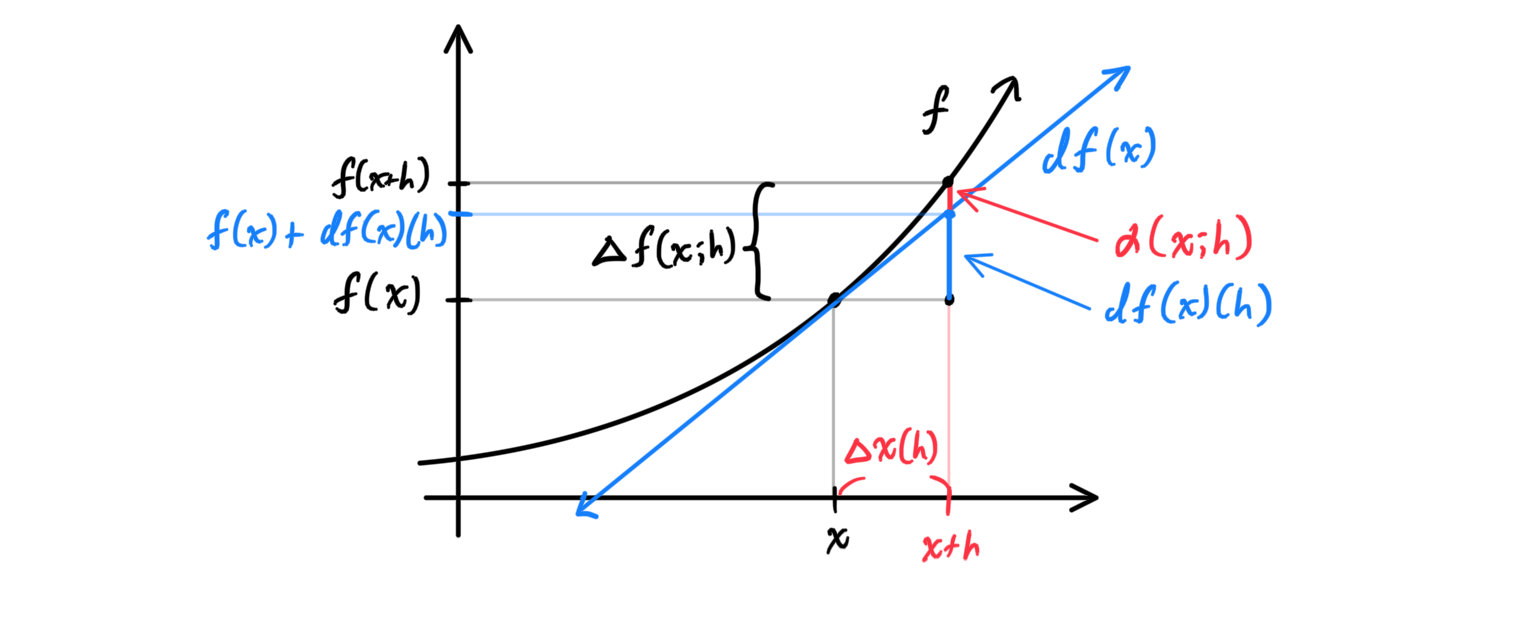
\includegraphics[scale=0.25]{img/Differential_Diagram.PNG}
    \end{center}
  \end{definition}

  \begin{definition}[Derivative]
    Given function $f: E \subset \mathbb{R} \longrightarrow \mathbb{R}$, the number
    \[f^\prime (x) = \lim_{h \rightarrow 0} \frac{f(x+h) - f(x)}{h}\]
    is called the \textbf{derivative} of the function $f$ at $x$. This equality can also be written in the equivalent form: 
    \[\frac{f(x+h) - f(x)}{h} = f^\prime (x) + \alpha (h)\]
    where $\alpha$ is infinitesimal as $h \rightarrow 0$. This also also equivalent to:
    \[f(x+h) - f(x) = f^\prime (x) h + o (h)\]
    where the error term $o(h) \rightarrow 0$ as $h \rightarrow 0$. 
  \end{definition}

  Note that we have defined the differentiability of a function at a point and the existence of its derivative at a point completely separately. But it turns out that the existence of this arbitrary number $f^\prime (x)$ we call the "derivative," defined
  \[f^\prime (x) = \lim_{h \rightarrow 0} \frac{f(x + h) - f(x)}{h}\]
  actually has an equivalent form of 
  \[f(x + h) - f(x) = f^\prime (x) h + o(h)\]
  But since $f^\prime(x)$ is in $\mathbb{R}$, the function $h \mapsto f^\prime (x) h$ is linear and $o(h)$ is infinitesimal, so it is in the form 
  \[f(x + h) - f(x) = df (x) (h) + \alpha(x; h)\]
  which, by definition, means that it is differentiable! Therefore, we have determined the equivalence between the differentiability of a function at a point and the existence of its derivative at the same point. Furthermore, this function $h \mapsto f^\prime (x) h$ is precisely the differential of $f$, meaning that
  \[df (x) (h) = f^\prime (x) h\]
  Furthermore, 
  \[\Delta f(x; h) - df(x)(h) = \alpha (x; h)\]
  and $\alpha(x;h) = o (h)$ as $h \rightarrow 0$, or in other words, the difference between the increment of the function and the value of the function $df(x)$ in $h$ is an infinitesimal of higher order than the first in $h$. For this reason, we say that the differential is the \textbf{principal linear part of the increment of the function}. 

  In particular, if $f(x) \equiv x$, then we have $f^\prime (x) \equiv 1$ and 
  \[dx (h) = 1 \cdot h = h\]
  Substituting this equality into $df(x) (h) = f^\prime (x) h$, we get
  \[df (x) (h) = f^\prime (x) \,dx (h)\]
  or without the input parameter $h$, 
  \[df(x) = f^\prime (x) \,dx\]
  Note that this is an equality between two functions of $h$. From this, we obtain the familiar \textbf{Leibniz notation} of the derivative: 
  \[\frac{df (x) (h)}{dx(h)} = f^\prime (x) \iff \frac{df(x)}{dx} = f^\prime (x)\]
  That is, the function $\frac{df(x)}{dx}$, which is the ratio of the functions $df(x)$ and $dx$, is constant and equals $f^\prime (x)$. 

  Let us try to construct successive approximations to an arbitrary function $f: E \longrightarrow \mathbb{R}$ at a given limit point $x_0$. That is, we find a function $g$ such that
  \[f = g + o(g)\]
  Depending on what $g$ is, we can construct better approximations of $f$. 

  \begin{example}[Constant Approximation]
    The 0th order approximation is when $g$ is a constant. That is, $g \equiv c_0$ for some $c_0 \in \mathbb{R}$. This means
    \begin{equation}
      f(x) = c_0 + o(c_0) = c_0 + o(1) \text{ as } x \rightarrow x_0
    \end{equation}
    More precisely, we want this difference $f(x) - c_0$ to be $o(1)$ as $x \rightarrow x_0$, which means that it is simply infinitesimal. Visualizing this, we can see that given a constant approximation (labeled in blue) to a function at $x_0$, its error term (labeled in green) is in fact, infinitesimal. All this boils down to the fact that 
    \[\lim_{x \rightarrow x_0} f(x) = c_0\]
    If the function is continuous at $x_0$, then 
    \[\lim_{x \rightarrow x_0} f(x) = f(x_0)\]
    and naturally $c_0 = f(x_0)$. Both the continuous (left) and noncontinuous case (right) is shown, but in most cases, we will assume continuity. 
    \begin{center}
      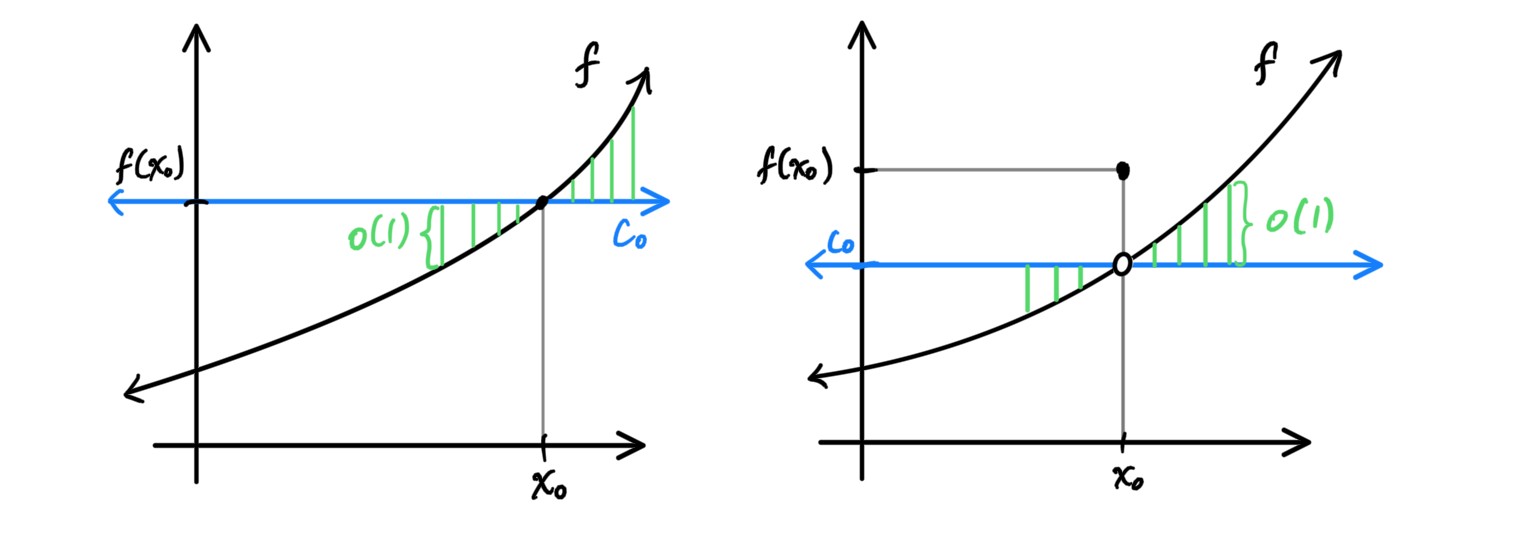
\includegraphics[scale=0.25]{img/Constant_Approximation_Continuous_Noncontinuous_case.PNG}
    \end{center}
  \end{example}

  \begin{example}[Linear Approximation]
    The 1st order approximation is a linear function that approximates $f$ as
    \begin{equation}
      f(x) = c_0 + c_1(x - x_0) + o(x - x_0) \text{ as } x \rightarrow x_0
    \end{equation}
    Following the previous logic, assuming $f$ continuous means that $c_0 = f(x_0)$. Furthermore, as $x \rightarrow x_0$
    \begin{align}
      f(x) = c_0 + c_1(x - x_0) + o(x - x_0) & \implies c_1 = \frac{f(x) - c_0 - o(x - x_0)}{x - x_0} \\
      & \implies c_1 = \frac{f(x) - c_0}{x - x_0} - \frac{o(x - x_0)}{x - x_0}\\
      & \implies c_1 = \frac{f(x) - c_0}{x - x_0} - o(1) \\
      & \implies c_1 = \lim_{x \rightarrow x_0} \frac{f(x) - c_0}{x - x_0} = f^\prime (x_0)
    \end{align}
    But this just means that $f^\prime (x_0) = c_1$, Note that before, we have proved the equivalence of the existence of a derivative at $x_0$ with differentiability at $x_0$ (which itself means that there exists a linear approximation $df(x)(h)$ that is a function of $h$). Here, we have created a linear approximation with respect to $x = x_0 + h$, rather than $h$ (shifted the function). 

    Therefore, the function 
    \[\alpha (x) = f(x_0) + f^\prime (x_0) (x - x_0)\]
    provides the best linear approximation to the function $f$ in a neighborhod of $x_0$ in the sense that for any other function $\beta(x)$ of the form 
    \[\beta(x) = c_0 + c_1 (x - x_0)\]
    we have $f(x) - \beta(x) \neq o(x - x_0)$ as $x \rightarrow x_0$. The graph of the function $\alpha$ is the straight line
    \[y - f(x_0) = f^\prime (x_0) (x - x_0)\]

    This leads to the definition of our familiar tangent line. 
  \end{example}

  \begin{definition}[Tangent Line]
    If a function $f: E \longrightarrow \mathbb{R}$ is differentiable at a point $x_0 \in E$, the line defined by
    \begin{equation}
      y - f(x_0) = f^\prime (x_0) (x - x_0)
    \end{equation}
    is called the \textbf{tangent} to the graph of $f$ at the point $(x_0, f(x_0))$. 
  \end{definition}

  Tangent spaces. 

  \begin{definition}[Tangent Space]
    Given function $f: E \longrightarrow \mathbb{R}$ and a point $x_0 \in E$, the increment of the argument $h = x - x_0$ can be regarded as a vector attached to the point $x_0$ and defining the transition from $x_0$ to $x_0 + h$. $h$ is called a \textbf{tangent vector}, and the set of all such vectors as $T_{x_0} \mathbb{R}$. Similarly, we denote $T_{y_0} \mathbb{R}$ the set of all displacement vectors from the point $y_0$ along the $y$-axis. 
    \begin{center}
        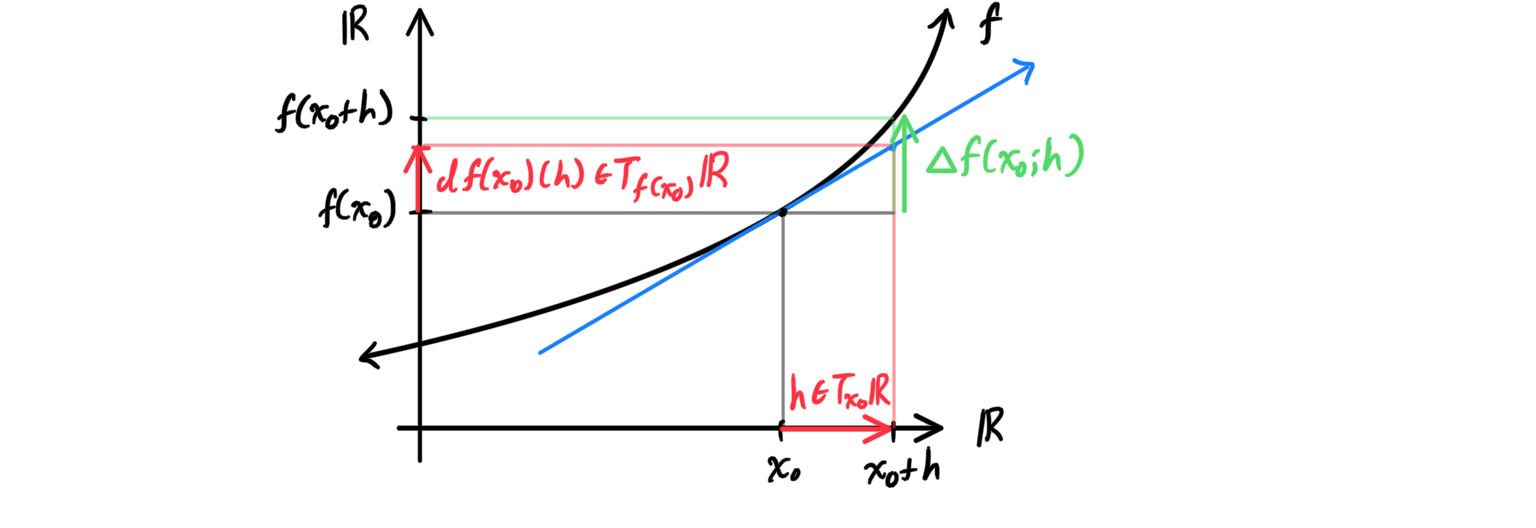
\includegraphics[scale=0.25]{img/Tangent_Space_1_dimensional_in_R.PNG}
    \end{center}
    Then, we can see that the differential is a mapping
    \[df(x_0): T_{x_0} \mathbb{R} \longrightarrow T_{f(x_0)} \mathbb{R}\]
    Note that that there are two functions to pay attention to here: 
    \begin{enumerate}
      \item The true increment of $f$, defined $h \mapsto f(x_0 + h) - f(x_0) = \Delta f(x_0; h)$ (labeled in green). 
      \item The differential $h \mapsto f^\prime (x_0) h = df(x_0) (h)$, which gives the increment of the tangent to the graph for increment $h$ in the argument (labeled in red). 
    \end{enumerate}
  \end{definition}

  \begin{example}
    Let $f(x) = \sin{x}$. Then we will show that $f^\prime (x) = \cos{x}$. 
    \begin{align*}
        \lim_{h \rightarrow 0} \frac{\sin{(x+h)} - \sin(x)}{h} & = \lim_{h \rightarrow 0} \frac{2 \sin \big( \frac{h}{2} \big) \cos \big( x + \frac{h}{2} \big)}{h} \\
        & = \lim_{h \rightarrow 0} \cos \Big( x + \frac{h}{2} \Big) \cdot \lim_{h\rightarrow 0} \frac{\sin\big( \frac{h}{2}\big)}{\big(\frac{h}{2}\big)} = \cos(x)
    \end{align*}
    Here, we have used the theorem on the limit of a product, the continuity of the function $\cos(x)$, the equivalence $\sin{t} \sim t$ as $t \rightarrow 0$, and the theorem on the limit of a composite function. 
  \end{example}

  \begin{example}
    We will show that $\cos^\prime (x) = - \sin(x)$. 
    \begin{align*}
        \lim_{h\rightarrow 0} \frac{\cos(x+h) - \cos(x)}{h} & = \lim_{h \rightarrow 0} \frac{-2 \sin \big(\frac{h}{2}\big) \, \sin \big( x + \frac{h}{2}\big)}{h} \\
        & = - \lim_{h\rightarrow 0} \sin \Big( x + \frac{h}{2} \Big) \cdot \lim_{h\rightarrow0} \frac{\sin\big(\frac{h}{2} \big)}{\big( \frac{h}{2} \big)} = -\sin(x)
    \end{align*}
  \end{example}


  \begin{lemma}[Differentiability Implies Continuity]
    If $f$ is differentiable at $x$, it is continuous at $x$. 
  \end{lemma}
  \begin{proof}
    Note that 
    \begin{equation}
      \text{Continuous at } \iff \lim_{y \to x} f(x) = 0 \iff \lim_{y \to x} f(x) - f(y) = 0
    \end{equation}
    So 
    \begin{equation}
      \lim_{y \to x} f(x) - f(y) = \lim_{y \to x} \frac{f(x) - f(y)}{x  - y} = 0
    \end{equation}
    and hence is continuous.
  \end{proof} 

  Therefore, we can see that the set of differentiable functions is a subset of the set of continuous functions.  

\subsection{Rules of Differentiation}

  \begin{lemma}[Arithmetic]
    If $f$ and $g$ are differentiable at $x$, then 
    \begin{enumerate}
      \item $f + g$ is differentiable at $x$ with 
        \begin{equation}
          (f + g)^\prime (x) = f^\prime (x) + g^\prime (x)
        \end{equation}
      \item $fg$ is differentiable at $x$ with 
        \begin{equation}
          (fg)^\prime = f^\prime (x) g(x) + f(x) g^\prime (x)
        \end{equation}
      \item $f/g$ is differentiable at $x$ with 
        \begin{equation}
          \bigg(\frac{f}{g}) \bigg)^\prime (x) = \frac{f^\prime(x) g(x) - f(x) g^\prime (x)}{g(x)^2}
        \end{equation}
    \end{enumerate}
  \end{lemma}
  \begin{proof}
    The proof for addition is pretty trivial, so we will prove for multiplication and division. For products, let's not take the quotient just yet. 
    \begin{equation}
      (fg)(x) - (fg)(y) = f(x) g(x) - f(y) g(y) 
    \end{equation}
    We know something about $f(x) - f(y)$ and $g(x) - g(y)$, so try to put it into this form. 
    \begin{equation}
      \big(f(x) - f(y) \big) g(x) + f(y) \big( g(x) - g(y) \big)
    \end{equation}
    Therefore, 
    \begin{equation}
      \frac{(fg)(x) - (fg) (y)}{x - y} = \underbrace{\frac{f(x) - f(y)}{x - y}}_{\text{exists}} g(x) + f(y) \underbrace{\frac{g(x) - g(y)}{x - y}}_{\text{exists}}
    \end{equation}
    So by taking limits, $f$ is continuous so $f(y) \to x$ as $y \to x$, and we finally have 
    \begin{equation}
      f^\prime (x) g(x) + f(x) g^\prime (x)
    \end{equation}
    For the quotient rule, it suffices to show from the product rule that $(1/g)^\prime (x) = - \frac{g^\prime (x)}{g(x)^2}$. 
  \end{proof}

  In proving properties of differentiability, it is useful to observe that 
  \begin{equation}
    \lim_{y \to x} \frac{f(x) - f(y)}{x - y} \iff f(x) - f(y) = (x - y) (f^\prime (x) + E)
  \end{equation}
  for some function $E$ where $\lim_{y \to x} E(x) = 0$. This is known as Taylor's formula. This is similar to the decomposition of sequences into a constant plus an infinitesimal sequence. 

  From this, we can find the derivative of polynomials. 

  \begin{corollary}[Polynomial Derivatives]
    The following are true. 
    \begin{enumerate}
      \item The derivative of a constant function is $0$
      \item The derivative of the identity function $f(x) = x$ is $1$. 
      \item The derivative of $f(x) = x^n$ is $n x^{n-1}$. 
      \item The derivative of a polynomial $f(x) = a_n x^n + \ldots  + a_0$ can then be found. 
    \end{enumerate}
  \end{corollary}
  \begin{proof}
    
  \end{proof}  

  \begin{theorem}[Chain Rule]
    Let $f: [a, b] \subset \mathbb{R} \to \mathbb{R}$ be a differentiable function, fix $x \in [a, b]$, and assume differentiable $g: I \to \mathbb{R}$ where $f(x) \in I$. Then, $h = g \circ f$ is differentiable at $x$ with the derivative 
    \begin{equation}
      h^\prime (x) = g^\prime (f(x)) f^\prime (x)
    \end{equation}
  \end{theorem}
  \begin{proof}
    We have 
    \begin{equation}
      g \big( f(x)\big) - g \big( f(y)\big) = \big( f(x) - f(y) \big) \big( g^\prime (f(x)) + E_{f(y) \to f(x)}\big)
    \end{equation}
    Now we divide by $x - y$. 
    \begin{equation}
      \frac{g(f(x)) - g(f(y))}{x - y} - \frac{f(x) - f(y)}{x - y} \cdot \big( g^\prime (f(x)) + E_{f(y) \to f(x)} \big)
    \end{equation}
    Now if $x \to y$, then $f$ is continuous, which implies $f(y) \to f(x)$ and so $E \to 0$, and so by taking this limit, the above evaluates to 
    \begin{equation}
      f^\prime (x) \cdot g^\prime (f(x))
    \end{equation} 
    We could have also done 
    \begin{equation}
      \frac{g(f(x)) - g(f(y))}{x - y} = \frac{g(f(x)) - g(f(y))}{f(x) - f(y)} \cdot \frac{f(x) - f(y)}{x  - y} \to g^\prime (f(x)) \cdot f^\prime (x) 
    \end{equation}
  \end{proof}

  \begin{theorem}[Differentiation of Inverse Functions over $\mathbb{R}$]
    Let $E_1, E_2 \subset \mathbb{R}$, and $f: E_1 \longrightarrow E_2$ and $f^{-1}: E_2 \longrightarrow E_1$ be mutually inverse and continuous at points $x_0 \in E_1$ and $f(x_0) = y_0 \in E_2$. If $f$ is differentiable at $x_0$ and $f^\prime(x_0) \neq 0$, then $f^{-1}$ also differentiable at the point $y_0$, and 
    \[\big(f^{-1}\big)^{-1} (y_0) = \big(f^\prime (x_0)\big)^{-1} \iff df^{-1} (y_0) = \big(df(x_0)\big)^{-1}\]

    \begin{figure}[H]
      \centering 
      \begin{tikzpicture}[scale=1.0]
        % Left plot - function f
        \begin{scope}
          % Axes
          \draw[->] (-1.5,0) -- (4,0) node[right] {$E_1$};
          \draw[->] (0,-1) -- (0,4) node[above] {$E_2$};
          
          % Function curve - smoother with more samples and tension
          \draw[thick] plot[domain=-1:3.5, samples=150, smooth, tension=0.9] 
              coordinates {(-1,0.5) (1,1.5) (3,4)};
          
          % Function label with direction arrow
          \node at (2.5,3.5) {$f$};
          
          % Mark point (x0, y0)
          \fill (1.5,2) circle (0.08);
          \draw[gray] (1.5,0) -- (1.5,2);
          \draw[gray] (0,2) -- (1.5,2);
          \node[below] at (1.5,0) {$x_0$};
          \node[left] at (0,2) {$y_0$};
          
          % Tangent line at (x0, y0)
          \draw[blue, thick, ->] (0,0.5) -- (3,3.5);
          \node[blue] at (3.5,2.5) {$f'(x_0)$};
        \end{scope}
        
        % Right plot - inverse function f^{-1}
        \begin{scope}[xshift=8cm]
          % Axes
          \draw[->] (-1.5,0) -- (4,0) node[right] {$E_2$};
          \draw[->] (0,-1) -- (0,4) node[above] {$E_1$};
          
          % Inverse function curve
          \draw[thick] plot[domain=-1:3.5, samples=100, smooth] 
              coordinates {(0.5, -1) (1.5, 1) (4, 3)};
          
          % Function label with direction arrow
          \node at (3.5,2) {$f^{-1}$};
          
          % Mark point (y0, x0)
          \fill (2,1.5) circle (0.08);
          \draw[gray] (2,0) -- (2,1.5);
          \draw[gray] (0,1.5) -- (2,1.5);
          \node[below] at (2,0) {$y_0$};
          \node[left] at (0,1.5) {$x_0$};
          
          % Tangent line at (y0, x0)
          \draw[blue, thick, ->] (0.5,0) -- (3.5,3);
          \node[blue] at (0.5,2.5) {$(f^{-1})'(x_0)=\frac{1}{f'(x_0)}$};
        \end{scope}
      \end{tikzpicture}
      \caption{Relationship between a function $f$ and its inverse $f^{-1}$, showing how their derivatives are related}
      \label{fig:function-inverse}
    \end{figure}

    Note that if we knew in advance that $f^{-1}$ was differentiable at $y_0$ (which is a stronger hypothesis), we can find immediately by the identity 
    \[(f^{-1} \circ f) (x) = x\]  
    and the theorem on the differentiation of a composite function that
    \[(f^{-1})^\prime (y_0) \cdot f^\prime (x_0) = 1\]
  \end{theorem}

  Note that if the hypothesis was satisfied, but $f^\prime (x_0) = 0$, then $f^{-1}$ would not be differentiable since it would have an undefined differential. 

  \begin{figure}[H]
    \centering 
    \begin{tikzpicture}[scale=1.3]
      % Left plot - function f with three points
      \begin{scope}
        % Axes
        \draw[->] (-2,0) -- (2,0) node[right] {$x$};
        \draw[->] (0,-2) -- (0,2) node[above] {$y$};

        \draw[<->, blue] (-1,1) -- (1,1) node[above] {$f^\prime (x_0) = 0$};
        
        % Connect the points with a smooth curve
        \draw[thick] plot[smooth, tension=0.9] coordinates {(-1,0) (0,1) (1,0)};
        
        % Function label
        \node at (0.5,0.2) {$f$};
      \end{scope}
      
      % Right plot - inverse function
      \begin{scope}[xshift=6cm]
        % Axes
        \draw[->] (-2,0) -- (2,0) node[right] {$y$};
        \draw[->] (0,-2) -- (0,2) node[above] {$x$};
        \draw[<->, blue] (1,-1) -- (1,1) node[right] {$(f^{-1})^\prime (x_0) = ?$};
        
        % Connect the points with a smooth curve (same tension)
        \draw[thick] plot[smooth, tension=0.9] coordinates {(0,-1) (1,0) (0,1)};
        
        % Function label
        \node at (0.2,0.5) {$f^{-1}$};
      \end{scope}
    \end{tikzpicture}
    \caption{A function through three points and its inverse relation}
    \label{fig:three-point-function-inverse}
  \end{figure}

\subsection{Basic Properties; Derivatives of Composite, Inverse Functions}

  \begin{theorem}[Arithmetic]
    If functions $f, g: E \longrightarrow \mathbb{R}$ are differentiable at a point $x \in E$, then 
    \begin{enumerate}
      \item their sum is differentiable at $x$, and 
      \[d(f+g) (x) = df(x) + dg(x) \iff (f+g)^\prime (x) = (f^\prime + g^\prime) (x)\]
      \item their product is differentiable at $x$, and 
      \[d (f \cdot g) (x) = g(x) df(x) + f(x) dg(x) \iff (f \cdot g)^\prime (x) = f^\prime (x) \cdot g(x) + f(x) \cdot g^\prime (x)\]
      \item their quotient is differentiable at $x$ if $g(x) \neq 0$, and 
      \[d \Big( \frac{f}{g} \Big) (x) =  \frac{g(x) df(x) - f(x) dg(x)}{g^2 (x)} \iff \bigg(\frac{f}{g}\bigg)^\prime (x) = \frac{f^\prime (x) g(x) - f(x) g^\prime (x)}{g^2 (x)}\]
    \end{enumerate}
    It is clear that $c\cdot df(x) = d (cf)(x)$, it is clear that the derivative is a linear operator from the space of all functions differentiable at $x_0$ the space of all functions. 
  \end{theorem}
  \begin{proof}
    Since $f$ and $g$ are differentiable at $x$, there exists the differential $df(x)(h) = f^\prime (x) h$ and $dg(x) = g^\prime (x) h$ where
    \begin{align*}
        f(x + h) & = f(x) + df(x)(h) + o(h) = f(x) + f^\prime (x) h + o(h) \\
        g(x + h) & = g(x) + dg(x)(h) + o(h) = g(x) + g^\prime (x) h + o(h) 
    \end{align*}
    From this relation, we can clearly see that a certain property of the differential automatically implies the same property of the derivative. (Remember that $f^\prime (x)$ and $g^\prime(x)$ are not functions! They are scalars defined on fixed point $x$.) 
    \begin{enumerate}
      \item Even though this derivation may be a bit long, every step is included to minimize ambiguity. 
      \begin{align*}
          (f + g)(x + h) - (f + g)(x) & = \big( f(x + h) + g(x + h)\big) - \big( f(x) + g(x)\big) \\
          & = \big( f(x + h) - f(x)\big) + \big(g(x + h) - g(x) \big) \\
          & = \big( df(x)(h) + o(h)\big) + \big( dg(x)(h) + o(h)\big) \\
          & = \big(f^\prime (x) h + o(h)\big) + \big( g^\prime (x) (h) + o(h)\big) \\
          & = \big(f^\prime(x) + g^\prime (x)\big) h + o(h) \\
          & = (f^\prime + g^\prime)(x)(h) + o(h) \\
          & = d (f + g)(x) h + o(h)
      \end{align*}
      \item For the product rule, we have
      \begin{align*}
          (f \cdot g) (x + h) & - (f \cdot g)(x) = f(x+h)g(x+h) - f(x) g(x) \\
          & = \big(f(x) + df(x) (h) + o(h)\big)\big(g(x) + dg(x)(h) + o(h)\big) - f(x) g(x) \\
          & = \big(f(x) + f^\prime (x) h + o(h)\big)\big(g(x) + g^\prime (x) h + o(h)\big) - f(x) g(x)
      \end{align*}
      Expanding this gives 
      \begin{multline*}
          \big(f^\prime (x) g(x) + f(x) g^\prime(x)\big) h + \big(f(x) + g(x)\big) o(h) + \\ f^\prime (x) g^\prime (x) h^2 + \big(f^\prime (x) + g^\prime (x) \big) h o(h) + \big(o(h)\big)^2
      \end{multline*}
      but note that since $f(x), g(x), f^\prime(x), g^\prime (x)$ are constants, we see that 
      \begin{enumerate}
        \item $\big(f(x) + g(x)\big) o(h) = o(h)$ because 
        \[\lim_{h \rightarrow 0} \frac{\big(f(x) + g(x)\big) o(h)}{h} = \big(f(x) + g(x)\big) \lim_{h \rightarrow 0} \frac{o(h)}{h} = 0\]
        \item $f^\prime(x) g^\prime (x) h^2 = o(h)$ since
        \[\lim_{h \rightarrow 0} \frac{f^\prime(x) g^\prime (x) h^2}{h} = f^\prime(x) g^\prime (x) \lim_{h \rightarrow 0}  h = 0\]
        \item $\big(f^\prime(x) + g^\prime(x)\big) h o(h) = o(h)$ because 
        \[\lim_{h \rightarrow 0} \frac{\big(f^\prime(x) + g^\prime(x)\big) h o(h)}{h} = \big(f^\prime(x) + g^\prime(x)\big) \lim_{h \rightarrow 0} o(h) = 0\]
        In fact, this term is of $o(h^2)$. 
        \item We can see that $(o(h))^2 = o(h)$ since 
        \[\lim_{h \rightarrow 0} \frac{(o(h))^2}{h} = \lim_{h \rightarrow 0} \frac{o(h)}{h} \cdot \lim_{h \rightarrow 0} o(h) = 0 \cdot 0 = 0\]
        In fact, $(o(h))^2 = o(h^2)$. 
      \end{enumerate}
      Therefore, the above simplifies to 
      \[(f \cdot g)(x + h) - (f \cdot g) (x) = \big(f^\prime(x) g(x) + f(x) g^\prime (x)\big) h + o(h)\]
      But this means that the differential (best approximation) $d(f \cdot g) (x)$ must be 
      \[(f \cdot g)^\prime (x) (h) = (f \cdot g)^\prime (x) h = \big(f^\prime(x) g(x) + f(x) g^\prime (x)\big) h\]
      \item Since the function $g(x) \neq 0$ at point $x$, then by continuity we can assume that there exists a neighborhood $U(x)$ where the image of that neighborhood does not vanish. That is, we can guarantee that $g(x + h) \neq 0$ for sufficiently small values of $h$. We assume $h$ is small in the following computations. 
      \begin{align*}
          \bigg(\frac{f}{g}\bigg) (x + h) - \bigg( \frac{f}{g}\bigg) (x) & = \frac{f(x + h)}{g(x + h)} - \frac{f(x)}{g(x)} \\
          & = \frac{1}{g(x)g(x + h)} \big( f(x + h) g(x) - f(x) g(x + h)\big) \\
          & = \bigg(\frac{1}{g^2(x)} + o(1)\bigg) \Big( \big(f(x) + f^\prime(x) h + o(h)\big) g(x) \\
          & \;\;\;\;\;\;\;\;\;\;\;\;\;\;\;\;\;\;\;\;\;\;\;\;\;\;\;\;\;\;\;- f(x) \big( g(x) + g^\prime(x) h + o(h)\big)\Big) \\
          & = \bigg(\frac{1}{g^2(x)} + o(1)\bigg) \Big(\big(f^\prime(x) g(x) - f(x) g^\prime(x)\big) h + o(h)\Big) \\
          & = \frac{f^\prime(x) g(x) - f(x) g^\prime(x)}{g^2 (x)} h + o(h)
      \end{align*}
      Note that here we have used the continuity of $g$ at the point $x$ and the fact that $g(x) \neq 0$ to deduce that
      \[\lim_{h \rightarrow 0} \frac{1}{g(x) g(x + h)} = \frac{1}{g^2(x)} \iff \frac{1}{g(x) + g(x + h)} = \frac{1}{g^2(x)} + o(1)\]
      where $o(1)$ is infinitesimal as $h \rightarrow 0$. 
    \end{enumerate}
  \end{proof}

  \begin{theorem}[Chain Rule]
    Let there be functions $f: E_1 \subset \mathbb{R} \longrightarrow E_2 \subset \mathbb{R}$ is differentiable at a point $x \in E_1$ and the function $g: E_2 \subset \mathbb{R} \longrightarrow \mathbb{R}$ is differentiable at point $y = f(x) \in E_2$, with respective differentials 
    \begin{align*}
        df(x)& : T_x \mathbb{R} \longrightarrow T_y \mathbb{R} \\
        dg(y)& : T_y\mathbb{R} \longrightarrow T_{g(y)} \mathbb{R}
    \end{align*}
    Then the composite function $g \circ f: E_1 \longrightarrow \mathbb{R}$ is differentiable at $x$, and $d(g \circ f)(x): T_x \mathbb{R} \longrightarrow T_{g \circ f(x)} \mathbb{R}$ is
    \[d(g \circ f)(x) = d g(y) \circ d f(x) \iff (g \circ f)^\prime (x) = g^\prime \big( f(x) \big) \circ f^\prime (x)\]
  \end{theorem}
  \begin{proof}
    We will denote the increment of the argument with the variables $h$ and $t$. Then, by differentiability of $f$ and $g$, we have
    \begin{align*}
        f(x + h) - f(x) & = f^\prime (x) h + o(h) \text{ as } h \rightarrow 0 \\
        g(y + t) - g(y) & = g^\prime(y) t + o(t) \text{ as } t \rightarrow 0
    \end{align*}
    Since the function $o(t)$ can be represented as $o(t) = \gamma(t) t$, where $\gamma = o(1)$ and hence is infinitesimal as $t \rightarrow 0$, meaning that we can assume $\gamma(0) = 0$ (since $o(t)$ is defined for $t = 0$). 

    We can think of the displacement of $x$ as like a chain reaction: As$x \mapsto x + h$, $f(x) \mapsto f(x + h)$, which we could interpret as $y \mapsto y + t$ and hence means that $g(y) \mapsto g(y + t)$. So, setting $f(x) = y$ and $f(x + h) = y + t$, by differentiability and hence continuity of $f$ at point $x$, we can conclude that $t \rightarrow 0$ as $h \rightarrow 0$. So, we have
    \[\gamma\big(f(x+h) - f(x)\big) = \gamma\big( (y+t) - y\big) = \gamma(t) = \alpha(h) \rightarrow 0 \text{ as } h \rightarrow 0\]
    Thus, we get 
    \begin{align*}
        o(t) = \gamma(t) t & = \gamma\big( f(x + h) - f(x)\big)\big( f(x + h) - f(x)\big) \\
        & = \alpha(h) \big(f^\prime(x) h + o(h)\big) \\
        & = \alpha(h) f^\prime(x) h + \alpha(h) o(h) \\
        & = o(h) + o(h) = o(h) \text{ as } h \rightarrow 0 \\
        (g \circ f)(x + h) - (g \circ f)(x) & = g\big(f(x + h)\big) - g\big(f(x)\big) \\
        & = g (y + t) - g(y) \\
        & = g^\prime (y) t + o(t) \\
        & = g^\prime \Big(f(x)\big) \big(f(x + h) - f(x)\big) + o\big( f(x + h) - f(x)\big) \\
        & = g^\prime \big(f(x)\big) \big(f^\prime (x) h + o(h)\big) + o\big( f(x + h)\big) - f(x)\big) \\
        & = g^\prime\big( f(x) \big) \big( f^\prime (x) h\big) + g^\prime \big( f(x)\big) \big(o(h)\big) + o\big(f(x + h) - f(x)\big) 
    \end{align*}
    Since $g^\prime\big(f(x)\big) \big( o(h)\big)$ is really just a constant multiplied by a function that is $o(h)$, it is $o(h)$. $o\big( f(x + h) - f(x) \big)$. As for $o\big(f(x + h) - f(x)\big)$, we see that since $f(x + h) - f(x) = t$, a function that is $o\big(f(x + h) - f(x)\big)$ becomes infinitesimal compared to $t$ as $t \rightarrow 0$. As already stated before, we have
    \[o\big(f(x + h) - f(x) \big) = o(h) \text{ as } h \rightarrow 0\]
    and thus, we proved that
    \begin{align*}
        (g \circ f)(x + h) - (g \circ f)(x) & = g^\prime (y) f^\prime (x) h + o(h) \\
        & = \big(dg(y) \circ df(x)\big) (h) + o(h)
    \end{align*}
  \end{proof}

\subsection{Theorems on Differentiability}

  \begin{theorem}[Local Extrema of Differentiable Functions Have Vanishing Derivative]
    Let $f: [a, b] \to \mathbb{R}$ and assume $f$ has a local maximum at $c \in (a, b)$ with $f$ differentiable at $c$. Then $f^\prime (c) = 0$. 
  \end{theorem}
  \begin{proof}
    If $y > c$ (with $y$ sufficiently close to $c$), then $f(c) \geq f(y)$ and so 
    \begin{equation}
      \implies \frac{f(c) - f(y)}{c - y} \leq 0 \implies \lim_{c - y} \frac{f(c) - f(y)}{c - y} = f^\prime (c) \leq 
    \end{equation}
    Similarly, if $y < c$, then $f^\prime (c) \geq 0$. So $f^\prime (c) = 0$. 
  \end{proof}

  Note that it is generally not true that $f^\prime (c) = 0$ if $c = a$ or $c = b$, i.e. at the endpoints. 

  \begin{theorem}[Rolle's Theorem]
    Suppose $f: [a, b] \to \mathbb{R}$ is differentiable on $(a, b)$. Then, if $f(a) = f(b)$, then there exists a $c \in (a, b)$ such that $f^\prime (c) = 0$. 
  \end{theorem}
  \begin{proof}
    Since $f$ is continuous on $[a, b]$, it has to attain its global max and min values somewhere in $[a, b]$. If either is in $(a, b)$, then the derivative is $0$. If max and min are attained on $\{a, b\}$, then since $f(a) = f(b)$, this implies that $f(x) = f(a)$ for all $x \in [a, b]$, which implies $f^\prime (x) = 0$. 
  \end{proof}

  \begin{theorem}[Mean Value Theorem]
    Assume $f: [a, b] \to \mathbb{R}$ is differentiable. Then there exists a $c \in (a, b)$ for which 
    \begin{equation}
      f^\prime (c) = \frac{f(b) - f(a)}{b - a} 
    \end{equation}
  \end{theorem}
  \begin{proof}
    Just use Rolle's on 
    \begin{equation}
      g(x) = f(x) - \bigg[ \frac{f(b) - f(a)}{b - a} + f(a) \bigg]
    \end{equation}
    which satisfies $g(a) = g(b) = 0$, and so there must exist some $c \in (a, b)$ such that $g^\prime (c) = 0$, i.e. 
    \begin{equation}
      f^\prime (c) - \frac{f(b) - f(a)}{b - a} = 0 \implies f^\prime (c) = \frac{f(b) - f(a)}{b - a}
    \end{equation}
  \end{proof} 

  Geometrically, this means that there exists a tangent line somewhere at $\zeta \in (a, b)$ that is parallel the secant line connecting the two points $\big(a, f(a)\big)$ and $\big( b, f(b)\big)$. 

  Some remarks: 
  \begin{enumerate}
    \item Physically, if $x$ is interpreted as time and $f(b) - f(a)$ as the amount of displacement over the time $b-a$ of a particle moving along the line, this theorem says that the velocity $f^\prime (x)$ of the particle at some time $\zeta \in (a, b)$ is such that if the particle had moved with constant velocity $f^\prime (\zeta)$ over the whole time interval, it would have been displaced by the same amount $f(b) - f(a)$. We call $f^\prime (\zeta)$ the \textbf{average velocity} over the time interval $[a, b]$. 
    \item Note that the Mean Value Theorem is important in that it connects the increment of a function over a finite interval with the derivative of the function on that interval. Up to now, we have characterized only the local (infinitesimal) increment of a function in terms of the derivative or differential at a given point. MVT connects the increment of a function over a \textbf{finite} interval with the derivative of the function. 
  \end{enumerate}

  The MVT actually leads to multiple useful corollaries. 

  \begin{corollary}[Derivative of a Monotonic Function]
    If the derivative of a function is nonnegative (resp. positive) at every point of an open interval, then the function is nondecreasing (resp. increasing) on that interval. 
  \end{corollary}
  \begin{proof}
    If $x_1 < x_2$ are two points of the interval, then the MVT
    \begin{equation}
      f(x_2) - f(x_1) = f^\prime (\zeta) (x_2 - x_1)
    \end{equation}
    shows that the sign of the left hand side must equal that of the right. 
  \end{proof}

  \begin{corollary}[Derivative of a Constant Function]
    A function that is continuous on a closed interval $[a,b]$ is constant on it if and only if its derivative equals $0$ at every point of the interval $[a,b]$ or the open interval $(a, b)$. 

    Therefore, if the derivatives $f_1^\prime (x)$ and $f_2^\prime (x)$ of two functions $f_1 (x)$ and $f_2 (x)$ are equal on some interval (that is, $f_1^\prime (x) = f_2^\prime (x)$ on the interval), then the difference
    \begin{equation}
      (f_1 - f_2) (x) = f_1 (x) - f_2 (x)
    \end{equation}
    is constant. 
  \end{corollary}
  \begin{proof}
    Given constant function $f$, the MVT equation 
    \begin{equation}
      0 = f(x_2) - f(x_1) = f^\prime (\zeta) (x_2 - x_1)
    \end{equation}
    implies that $f^\prime (\zeta) = 0$ for all $x_1, x_2 \in E$. It follows that by the arithmetic properties of the derivative, given two functions $f_1, f_2$ with the same derivative on an interval, the derivative of their difference $(f_1 - f_2)^\prime = 0$, and therefore must be constant on that interval. 
  \end{proof}

  The following proposition is a useful generalization of Lagrange's theorem. 

  \begin{theorem}[Cauchy's Finite-Increment Theorem]
    Let $x = x(t)$ and $y = y(t)$ be functions that are continuous on a closed interval $[\alpha, \beta]$ and differentiable on the open interval $(\alpha, \beta)$. Then, there exists a point $\tau \in [\alpha, \beta]$ such that
    \begin{equation}
      x^\prime (\tau) \big( y(\beta) - y (\alpha)\big) = y^\prime (\tau) \big( x(\beta) - x(\alpha)\big)
    \end{equation}
    If in addition $x^\prime (t) \neq 0$ for each $t \in (\alpha, \beta)$, then $x(\alpha) \neq x(\beta)$ and we have the equality 
    \begin{equation}
      \frac{y(\beta) - y(\alpha)}{x(\beta) - x(\alpha)} = \frac{y^\prime (\tau)}{x^\prime (\tau)}
    \end{equation}
  \end{theorem}

  \begin{corollary}[Taylor's Theorem of 2nd Order]
    If $f$ is twice differentiable on $[a, b]$, then 
    \begin{equation}
      f(b) - f(a) = (b - a) f^\prime (b) + \frac{(b-a)^2}{2} f^{\prime \prime} (c)
    \end{equation}
    for some $c \in (a, b)$. 
  \end{corollary} 

  \begin{theorem}
    Suppose $f: [a, b] \to \mathbb{R}$ is a real and differentiable function and suppose $f^\prime (a) < \lambda < f^\prime (b)$. Then there exists $x \in (a, b)$ such that $f^\prime (x) = \lambda$.\footnote{i.e. $f$ doesn't have to be continuous, but it must have a middle value.}
  \end{theorem}
  \begin{proof}
    Let $g(x) = f(x) - \lambda x$. Then $g$ is differentiable with $g^\prime (x) = f^\prime (x) - \lambda$. But this implies that
    \begin{align}
      g^\prime (a) & = f^\prime (a) - \lambda < 0 \implies \exists t_1 \in (a, b) \text{ s.t. } g(a) > g(t_1) \\
      g^\prime (b) & = f^\prime (b) - \lambda > 0 \implies \exists t_2 \in (a, b) \text{ s.t. } g(b) > g(t_2) 
    \end{align}
    and by the mean value theorem there exists $x \in (a, b)$ s.t. $g^\prime (x) = 0 \implies f^\prime (x) = \lambda$. 
  \end{proof}

  \begin{example}
    A counterexample is $f(x) = |x|$. 
  \end{example}

  That is, the derivative of a differentiable function cannot ``jump,'' so it's like the IVT of derivatives. 

  \begin{corollary}
    You can't have a jump discontinuity for derivatives. 
  \end{corollary}

  \begin{theorem}[L'Hopital's Rule]
    Suppose $f, g$ are continuously differentiable functions with $f(c) = g(c) = 0$ and $g^\prime (c) \neq 0$. Then, 
    \begin{equation}
      \lim_{x \to c} \frac{f(x)}{g(x)} = \lim_{x \to c} \frac{f^\prime (x)}{g^\prime (x)}
    \end{equation}
  \end{theorem}
  \begin{proof}
    We have 
    \begin{align}
      \lim_{x \to c} \frac{f(x)}{g(x)} & = \lim_{x \to c} \frac{f(x) - f(c)}{g(x) - g(c)} \\ 
                                       & = \lim_{x \to c} \frac{\frac{f(x) - f(c)}{x -  c}}{\frac{g(x) - g(c)}{x - c}} \\ 
                                       & = \frac{\lim_{x \to c} \frac{f(x) - f(c)}{x - c}}{\lim_{x \to c} \frac{g(x) - g(c)}{x - c}} \\ 
                                       & = \lim_{x \to c} \frac{f^\prime (x)}{g^\prime (x)}
    \end{align}
  \end{proof}

  \begin{example}
    Let $f(x) = \sin{x}$ and $g(x) = -0.5x$. Then, the function 
    \begin{equation}
      h(x) = \frac{f(x)}{g(x)} = \frac{\sin{x}}{-0.5x}
    \end{equation}
    is clearly undefined at $x = 0$. 
    However, we can solve the limit using L'Hopital's rule to get
    \begin{equation}
      \lim_{x \rightarrow 0} \frac{\sin{x}}{-0.5x} = \lim_{x \rightarrow 0} \frac{\cos{x}}{-0.5} = -2
    \end{equation}
    Therefore, $h: \mathbb{R} \setminus 0 \longrightarrow \mathbb{R}$ can be completed to continuous function on all of $\mathbb{R}$ by defining the extension: 
    \begin{equation}
      H(x) \equiv \begin{cases} h(x), & x \neq 0 \\ -2, & x = 0 \end{cases} 
    \end{equation}
  \end{example}

\subsection{Higher Order Derivatives} 

  We can continue this pattern to get a quadratic approximation of $f$ in the form
  \[f(x) = c_0 + c_1 (x - x_0) + c_2 (x - x_0)^2 + o\big((x - x_0)^2 \big) \text{ as } x \rightarrow x_0\]
  As we have done in the previous subsection, we can derive (assuming continuity of $f$) $c_0 = f(x_0), c_1 = f^\prime (x_0)$. To derive what $c_2$ should be, we see that the equation above implies
  \[c_2 = \frac{f(x) - c_0 - c_1 (x - x_0) - o\big((x - x_0)^2 \big)}{(x - x_0)^2} = \frac{f(x) - c_0 - c_1 (x - x_0)}{(x - x_0)^2} - o(1)\]
  which means
  \[c_2 = \lim_{x \rightarrow x_0} \frac{f(x) - c_0 - c_1 (x - x_0)}{(x - x_0)^2}\]
  Extending this, if we are seeking a polynomial $P_n(x_0; x) = c_0 + c_1 (x - x_0) + \ldots + c_n (x - x_0)^n$ such that
  \[f(x) = c_0 + c_1 (x - x_0) + \ldots + c_n (x - x_0)^n + o\big((x - x_0)^n\big) \text{ as } x \rightarrow x_0\]
  we would find 
  \begin{align*}
      c_0 & = \lim_{x \rightarrow x_0} f(x) \\
      c_1 & = \lim_{x \rightarrow x_0} \frac{f(x) - c_0}{x - x_0} \\
      c_2 & = \lim_{x \rightarrow x_0} \frac{f(x) - c_0 - c_1 (x - x_0)}{(x - x_0)^2} \\
      \ldots & = \ldots \\
      c_n & = \lim_{x \rightarrow x_0} \frac{f(x) - (c_0 + \ldots + c_{n-1}(x - x_0)^{n-1})}{(x - x_0)^n}
  \end{align*}

  We formalize the order of these approximations by analyzing their error bound. 

  \begin{definition}[nth Order Contact]
    If $f, g: E \longrightarrow \mathbb{R}$ are continuous at point $x_0$ and $(f - g) (x) = o\big( (x - x_0)^n \big)$ as $x \rightarrow x_0$, then we say that $f$ and $g$ have \textbf{$n$th order contact at $x_0$}, or more precisely, \textbf{contact of order at least $n$}. 

    The following visual shows approximations $g$ of an arbitrary function $f$ that have $0$th (left), $1$st (middle), and $2$nd (right) order contact at $x_0$. 
    \begin{center}
        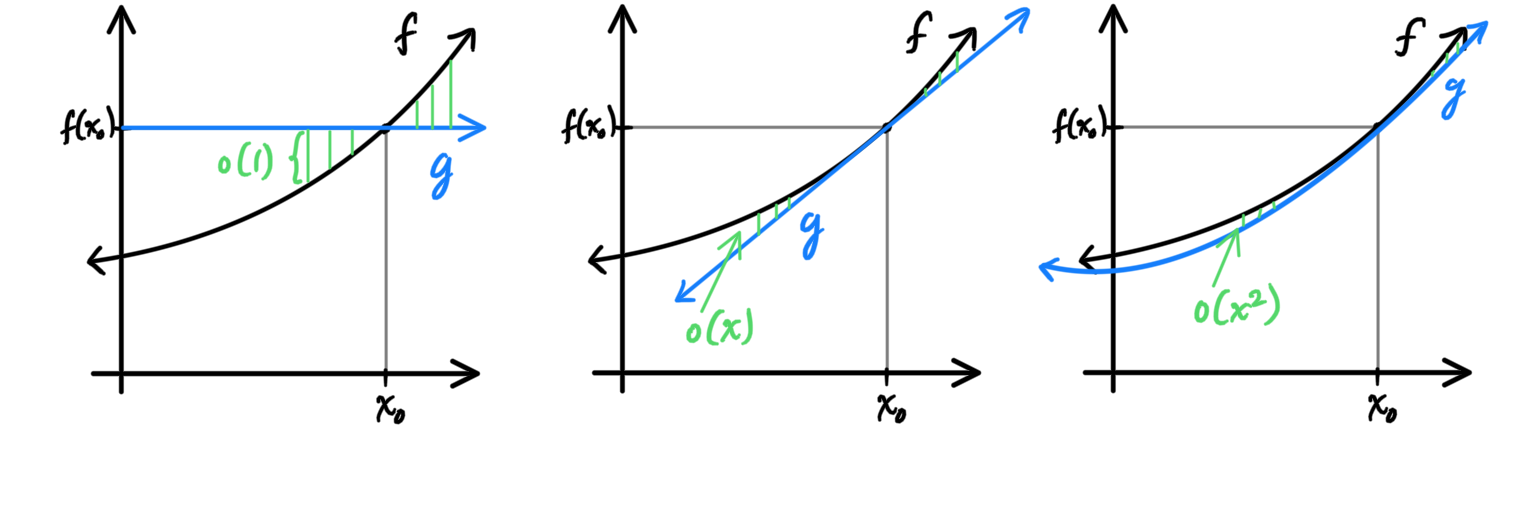
\includegraphics[scale=0.25]{img/nth_order_contact.PNG}
    \end{center}
  \end{definition}

  \begin{lemma}[Leibniz' Formula]
    Let $u(x)$ and $v(x)$ be functions having derivatives up to order $n$ inclusive on a common set $E$. Then, 
    \[(uv)^{(n)} = \sum_{m = 0}^n \binom{n}{m} u^{(n-m)} v^{(m)}\]
    This means that given a polynomial $P_n (x) = c_0 + c_1 (x - x_0) + \ldots + c_n (x - x_0)^n$, then 
    \begin{align*}
        P_n(x_0) & = 0 \\
        P_n^\prime (x_0) & = 1! c_1 \\
        P_n^{\prime\prime} (x_0) & = 2! c_2 \\
        \ldots & = \ldots \\
        P_n^{(n)} (x_0) & = n! c_n \\
        P_n^{(k)} (x_0) & = 0 \text{ for } k > n
    \end{align*}
    and thus the polynomial $P_n (x)$ can be written as
    \[P_n (x) = P_n^{(0)} (x_0) + \frac{1}{1!} P_n^{(1)} (x_0) (x-x_0) + \frac{1}{2!} P_n^{(2)} (x_0) (x-x_0)^2 + \ldots + \frac{1}{n!} P_n^{(n)} (x_0) (x-x_0)^n\]
  \end{lemma}


  \begin{theorem}[Taylor's Theorem]
    Suppose $f: [a, b] \to \mathbb{R}$, $n$ is a positive integer, $f^{(n-1)}$ is continuous on $[a, b]$, and $f^{(n)} (t)$ exists for every $t \in (a, b)$. Let $\alpha < \beta$ be distinct points of $[a, b]$, and define 
    \begin{equation}
      P(t) \coloneqq \sum_{k=0}^{n-1} \frac{f^{(k)}(\alpha)}{k!} (t - \alpha)^k 
    \end{equation}
    Then, there exists a point $x \in (\alpha, \beta)$ such that 
    \begin{equation}
      f(\beta) = P(\beta) + \frac{f^{(n)}(x)}{n!} (\beta - \alpha)^n 
    \end{equation}
  \end{theorem}

\subsubsection{Taylor's Formula}

  From the following results one may deduce that the more derivatives of two functions coincide (including the derivative of the $0$th order) at a point, the better these functions approximate each other in a neighborhood of that point. Using Leibniz's rule, approximations up to a certain degree at a point can be expressed as a polynomial 
  \[P_n (x_0; x) = P_n (x_0) + \frac{P_n^\prime (x_0)}{1!} (x-x_0) + ... + \frac{P_n^{(n)} (x_0)}{n!} (x-x_0)^n\]
  where each coefficient of the polynomial 

  \begin{definition}[Taylor Polynomial]
    If a function $f:E \longrightarrow \mathbb{R}$ has derivatives of all orders $n \in \mathbb{N}$ at a point $x_0$, the unique series
    \[P_n (x_0; x) = f(x_0) + \frac{f^\prime (x_0)}{1!} (x-x_0) + ... + \frac{f^{(n)} (x_0)}{n!} (x-x_0)^n\]
    is the \textbf{Taylor polynomial of order $n$ of $f(x)$ at $x_0$}. We can see that the derivatives of $f$ and $P_n$ coincide up to order $n$. 
  \end{definition}

  \begin{definition}[Analytic Functions]
    We cannot assume that the Taylor series of an infinitely differentiable function converges to the function $f$ within a neighborhood $U(x_0)$, nor can we assume that it converges at all! These types of "nice" functions that have a Taylor approximation within the neighborhood of $x_0$ are called \textbf{analytic functions} and can be written in the form 
    \[f(x) =  f(x_0) + \frac{f^\prime (x_0)}{1!} (x-x_0) + ... + \frac{f^{(n)} (x_0)}{n!} (x-x_0)^n + r_n (x_0; x)\]
    where $r$ is called the \textbf{remainder term}. 
  \end{definition}

  \begin{example}[Infinitely Differentiable, Non-Analytic Function]
    A example of a non-analytic function is
    \begin{equation}
      f(x) = \begin{cases} e^{-1/x^2} & \text{ if } x \neq 0 \\ 0 & \text{ if } x = 0 \end{cases}
    \end{equation}
    which looks like the following. 

    \begin{figure}[H]
      \centering 
      \begin{tikzpicture}[scale=1.5]
        % Draw the coordinate axes
        \draw[->] (-3.5,0) -- (3.5,0) node[right] {$x$};
        \draw[->] (0,0) -- (0,1.5) node[above] {$y$};
        
        % Draw tick marks
        \foreach \x in {-1,1}
          \draw (\x,0.1) -- (\x,-0.1) node[below] {$\x$};
        
        % Draw the function y = e^(-1/x²)
        \draw[blue, thick, domain=-3:-0.01, samples=100, smooth] 
          plot (\x, {exp(-1/(\x*\x))});
        \draw[blue, thick, domain=0.01:3, samples=100, smooth] 
          plot (\x, {exp(-1/(\x*\x))});
        
        % Add function label
        \node[blue] at (2,1) {$y = e^{-\frac{1}{x^2}}$};
        
        % Add horizontal asymptote at y=0
        \draw[gray, dashed] (-3.5,0) -- (3.5,0);
      \end{tikzpicture}
      \caption{Graph of the function $y = e^{-\frac{1}{x^2}}$. This function equals $0$ at $x=0$ and approaches $1$ as $|x|$ approaches infinity. One can verify that the derivative $f^{(k)} (0) = 0$ for all $k$ and hence the Taylor series is identically equal to $0$, while $f(x) \neq 0$ if $x \neq 0$. }
      \label{fig:bump-function}
    \end{figure}
  \end{example}

  The relationship between these different conditions is nicely summarized in the figure. 
  \begin{center}
  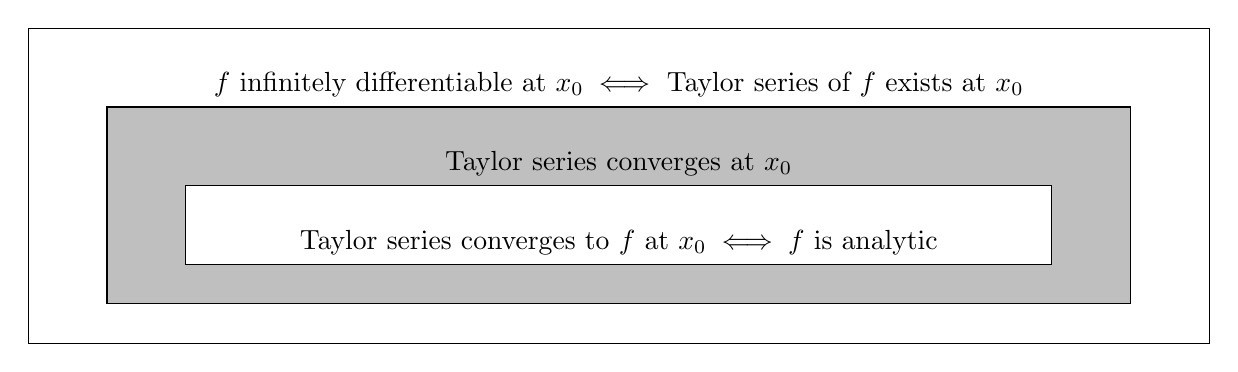
\begin{tikzpicture}
      \draw (-7.5,0) rectangle (7.5, 4);
      \draw[fill=lightgray] (-6.5, 0.5) rectangle (6.5, 3);
      \draw[fill=white] (-5.5, 1) rectangle (5.5, 2);
      \node[above] at (0, 1) {Taylor series converges to $f$ at $x_0 \iff f$ is analytic};
      \node[above] at (0, 2) {Taylor series converges at $x_0$};
      \node[above] at (0, 3) {$f$ infinitely differentiable at $x_0 \iff $ Taylor series of $f$ exists at $x_0$};
  \end{tikzpicture}
  \end{center}

  The following lemma proves why Taylor Polynomials are considered a "good" approximations to analytic functions. 

  \begin{lemma}[Infinitesimality of Functions with Vanishing Derivative up to Order $n$]
    Given a function $\varphi: E \longrightarrow \mathbb{R}$ defined on a closed interval $E$ with endpoint $x_0$, let its derivatives vanish up to order $n$ at $x_0$. That is
    \[\varphi(x_0) = \varphi^\prime (x_0) = \ldots = \varphi^{(n)} (x_0) = 0\]
    Then, $\varphi = o\big((x - x_0)^n\big)$ as $x \rightarrow x_0$. 
  \end{lemma}
  \begin{proof}
  We prove by induction. For $n = 1$, the definition of differentiability states that 
  \[\varphi(x) = \varphi^(x_0) + \varphi^\prime (x - x_0) + o(x - x_0) \text{ as } x \rightarrow x_0\]
  and so we have proved that 
  \[\varphi(x_0) = \varphi^\prime (x_0) = 0 \implies \varphi(x) = o(x - x_0) \text{ as } x \rightarrow x_0\]
  Now, suppose this assertion has been proved for order $n = k - 1 \geq 1$. That is, we have shown that 
  \[\varphi(x_0) = \ldots = \varphi^{(k-1)}(x_0) = 0 \implies \varphi= o\big((x - x_0)^{k-1}\big) \text{ as } x \rightarrow x_0\]
  Then we must show that this is valid for order $n = k \geq 2$. Assume that 
  \[\varphi(x_0) = \varphi^\prime (x_0) = \ldots = \varphi^{(k)} (x_0) = 0\]
  We can see that this is equivalent to
  \[(\varphi^\prime)^\prime (x_0) = (\varphi^\prime)^{(2)} (x_0) = \ldots = (\varphi^\prime)^{(k-1)} = 0\]
  and therefore by the induction assumption, we have
  \[\varphi^\prime = o\big( (x - x_0)^{k-1}\big) \text{ as } x \rightarrow x_0\]
  which means that we can put it in form 
  \[\varphi(x) = \alpha (x) (x - x_0)^{k-1} \text{ so that } \lim_{x \rightarrow x_0} \varphi(x) = \lim_{x \rightarrow x_0} \alpha(x) = 0 \]

  From the mean value theorem and substituting what we have above, we get 
  \begin{align*}
      \varphi(x) = \varphi(x) - \varphi(x_0) & = \varphi^\prime(\zeta) (x - x_0) \\
      & = \varphi (\zeta) (\zeta - x_0)^{k-1} (x - x_0)
  \end{align*}
  where $\zeta \in (x_0, x)$. However, this implies that $|\zeta - x_0| < |x - x_0|$, and thus, as $x \rightarrow x_0$, $\zeta \rightarrow x_0$, which then makes $\alpha(\zeta) \rightarrow 0$. Since
  \[|\varphi (x)| \leq |\alpha(\zeta)| |x - x_0|^{k-1} |x - x_0| = |\alpha(\zeta)| |x - x_0|^k\]
  This means that $\varphi(x)$ is bounded by function $|\alpha(\zeta)| |x - x_0|^k$, which is $o\big((x-x_0)^k\big)$, and so 
  \[\varphi = o\big( (x - x_0)^k \big) \text{ as } x \rightarrow x_0\]
  By induction, this works for all orders $n$. 
  \end{proof}

  \begin{theorem}[Peano's Form of the Remainder]
  Given analytic function $f: E \longrightarrow \mathbb{R}$, a point $x_0 \in E$, and its $n$th order Taylor polynomial $P_n (x_0; x)$ around $x_0$, $P_n$ is a "good" approximation of $f$ in the fact that its error term is $o\big((x - x_0)^n\big)$. That is, 
  \[f(x) = P_n (x_0; x) + o\big((x - x_0)^n \big) \text{ as } x \rightarrow x_0\]
  This equation where $r_n (x; x_0) = o\big((x - x_0)^n\big)$ is called the \textbf{Peano's form of the remainder}. 
  \end{theorem}
  \begin{proof}
  Since the Taylor polynomial $P_n (x_0; x)$ is constructed from the requirement that its derivatives up to order $n$ inclusive must coincide with the corresponding derivatives of $f$ at $x_0$, it follows that
  \[r_n (x_0; x_0) \equiv f^{(k)} (x_0) - P_n^{(k)} (x_0; x_0) = 0 \text{ for } k = 0, 1, \ldots, n\]
  Using the previous lemma, a this means that $r_n (x; x_0) = o\big((x - x_0)^n\big)$ as $x \rightarrow x_0$. 
  \end{proof}

  \begin{theorem}[Lagrange Form of the Remainder]
  If $f: E \longrightarrow \mathbb{R}$ has derivatives of order $n+1$ on the open interval with endpoints $x_0$ and $x$, then 
  \[f(x) = f(x_0) + \frac{f^\prime (x_0)}{1!} (x - x_0) + \ldots + \frac{f^{(n)}(x_0)}{n!} (x - x_0)^n + r_n (x; x_0)\]
  where 
  \[r_n (x; x_0) = \frac{f^{(n+1)} (\zeta)}{(n+1)!} (x - x_0)^{n+1}\]
  This form is called \textbf{Taylor's formula with the Lagrange form of the remainder}. Furthermore, this form says that if $f^{(n+1)} (x)$ is bounded in a neighborhood of $x_0$, it also implies the formula
  \[f(x) = f(x_0) + \frac{f^\prime (x_0)}{1!} (x - x_0) + \ldots + \frac{f^{(n)} (x_0)}{n!} (x - x_0)^n + O\big( (x - x_0)^{n+1} \big)\]
  Therefore, we can use this boundedness of $f^{(n+1)}$ to find the maximum error bound 
  \[|r_n (x; x_0)|\]
  of $P_n (x; x_0)$. 
  \end{theorem}
  \begin{proof}
  It is a direct result from the lemma. This is actually a generalization of the mean value theorem but for higher orders. 
  \end{proof}

  \begin{corollary}[Table of Asymptotic Formulas for Elementary Functions]
  We write the Maclaurin series (Taylor series around $x = 0$) for elementary functions. Note that these error terms are $O(x^{n+1})$ (bounded compared to $x^{n+1}$) and $o(x^n)$ (infinitesimal compared to $x^n$). 
  \begin{align*}
      e^x & = 1 + \frac{1}{1!} x + \frac{1}{2!} x^2 + \ldots + \frac{1}{n!} x^n + O(x^{n+1}) \\
      \cos{x} & = 1 - \frac{1}{2!} x^2 + \frac{1}{4!}x^4 - \ldots + \frac{(-1)^n}{(2n)!} x^{2n} + O(x^{2n+2}) \\
      \sin{x} & = x - \frac{1}{3!} x^3 + \frac{1}{5!}x^5 - \ldots + \frac{(-1)^n}{(2n+1)!} x^{2n+1} + O(x^{2n+3}) \\
      \cosh{x} & = 1 + \frac{1}{2!} x^2 + \frac{1}{4!} x^4 + \ldots + \frac{1}{(2n)!} x^{2n} + O(x^{2n+2}) \\
      \sinh{x} & = x + \frac{1}{3!} x^3 + \frac{1}{5!} x^5 + \ldots + \frac{1}{(2n+1)!} x^{2n+1} + O(x^{2n+3}) \\
      \ln{(1+x)} & = x - \frac{1}{2}x^2 + \frac{1}{3} x^3 - \ldots + \frac{(-1)^n}{n} x^n + O(x^{n+1}) \\
      (1 + x)^\alpha & = 1 + \frac{\alpha}{1!} x + \frac{\alpha(\alpha-1)}{2!} x^2 + \ldots + \frac{\alpha (\alpha-1) \ldots (\alpha - n + 1)}{n!} x^n + O(x^{n+1})
  \end{align*}
  \end{corollary}

\subsection{Derivatives of Special Functions}

  We can now connect the concepts of derivatives and monotonicity. 

  \begin{theorem}[Derivative $\implies$ Monotonicity]
    Given function $f: E \longrightarrow \mathbb{R}$ that is differentiable on an open interval $(a, b) = E$, 
    \begin{align*}
      f^\prime (x) > 0 & \implies f \text{ is increasing} \\
      f^\prime (x) \geq 0 & \iff f \text{ is nondecreasing} \\
      f^\prime (x) \equiv 0 & \iff f \text{ is constant} \\
      f^\prime (x) \leq 0 & \iff \text{ is nonincreasing} \\
      f^\prime (x) < 0 & \implies f \text{ is decreasing} 
    \end{align*}
    Note that if $f$ is strictly increasing (resp. decreasing), we cannot determine that $f^\prime(x) \geq 0$ (resp. $f^\prime (x) \leq 0$).\footnote{For example, take the function $f(x) = x^3$, which is strictly increasing, but has derivative $f^\prime (0) = 0$ at $x = 0$.} It is clearly strictly increasing within a neighborhood $U(0)$, so we can see that
    \begin{align*}
      f \text{ is increasing} & \implies f^\prime (x) \geq 0 \\
      f \text{ is decreasing} & \implies f^\prime (x) \leq 0
    \end{align*}
  \end{theorem}

  Similarly, we can connect the concepts of extrema and derivatives. 

  \begin{theorem}[First Derivative Test]
    Let function $f: E \longrightarrow \mathbb{R}$ be defined in a neighborhood $U(x_0)$ of point $x_0$, which is continuous at $x_0$ and differentiable in $\mathring{U}(x_0)$, a deleted neighborhood of $x_0$. (Note that this is broader hypothesis than just assuming that $f$ be differentiable at $x_0$.) Let
    \[\mathring{U}^- (x_0) \equiv \{x \in U(x_0) \;|\; x < x_0\}, \;\; \mathring{U}^+ (x_0) \equiv \{x \in U(x_0) \;|\; x > x_0\}\]
    That is, $\mathring{U}^- (x_0)$ is the left portion of $\mathring{U}(x_0)$ and $\mathring{U}^+ (x_0)$ is the right portion of $\mathring{U}(x_0)$. Then, 
    \begin{enumerate}
      \item $(x_0, f(x_0))$ is strict local minimum if $f^\prime(x) < 0$ in $\mathring{U}^- (x_0)$ and $f^\prime (x) > 0$ in $\mathring{U}^+ (x_0)$. 

      \item $(x_0, f(x_0))$ is strict local maximum if $f^\prime(x) > 0$ in $\mathring{U}^- (x_0)$ and $f^\prime (x) < 0$ in $\mathring{U}^+ (x_0)$. 

      \item $(x_0, f(x_0))$ has no extremum at $x_0$ if $f^\prime (x) > 0$ in both $\mathring{U}^- (x_0), \mathring{U}^+ (x_0)$, or if $f^\prime(x)< 0$ in both $\mathring{U}^- (x_0), \mathring{U}^+ (x_0)$. 
    \end{enumerate}
  \end{theorem}

  Note that if there is a discontinuity at a point $x_0$, then this theorem does not apply. For example, $(x_0, f(x_0))$ in the graph below is a local minimum, even though the derivatives to the left of $x_0$ are positive and those to the right of $x_0$ are negative (within neighborhood $U(x_0)$). Similarly, $(x_0, g(x_0))$ is a local maximum, even though the derivative to the left and to the right of $x_0$ are both positive. 
  \begin{center}
      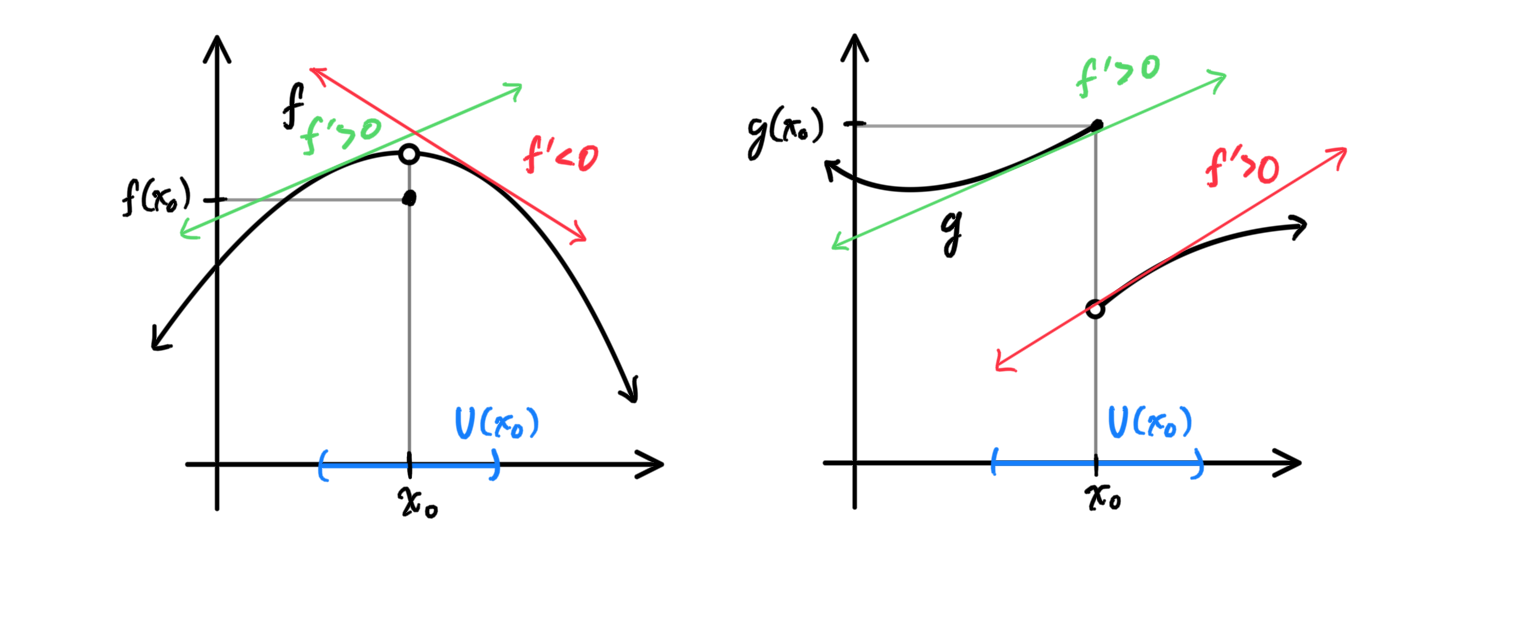
\includegraphics[scale=0.3]{img/Theorem_not_apply_if_Discontinuity.PNG}
  \end{center}

  \begin{proposition}[2nd, $n$th Derivative Test]
    Let function $f: E \longrightarrow \mathbb{R}$ be defined on a neighborhood $U(x_0)$ of $x_0$ has derivatives of order up to $n$ inclusive at $x_0$. If its derivatives up to the $(n-1)$th order vanishes 
    \[f^\prime (x_0) = f^{\prime\prime} (x_0) ... = f^{(n-1)} (x_0) = 0\]
    but the $n$th derivative at $x_0$ does \textbf{not} vanish
    \[f^{(n)} (x_0) \neq 0\]
    then 
    \begin{enumerate}
      \item $n$ is odd $\implies$ there is no local extremum at $x_0$ 
      \item $n$ is even $\implies$ there is a local extremum at $x_0$
      \begin{enumerate}
        \item $f^{(n)} (x_0) > 0 \implies$ it is a strict local minimum
        \item $f^{(n)} (x_0) < 0 \implies$ it is a strict local maximum
      \end{enumerate}
    \end{enumerate}
  \end{proposition}

  \begin{definition}[Convex, Concave Functions]
    A function $f: (a, b) \longrightarrow \mathbb{R}$ defined on an open interval $(a, b) \subset \mathbb{R}$ is \textbf{convex} if the inequality
    \[f( \alpha_1 x_1 + \alpha_2 x_2) \leq \alpha_1 f(x_1) + \alpha_2 f(x_2)\]
    holds and \textbf{concave}, or \textbf{convex upward}, if the inequality 
    \[f( \alpha_1 x_1 + \alpha_2 x_2) \geq \alpha_1 f(x_1) + \alpha_2 f(x_2)\]
    holds for all pairs of points $x_1, x_2 \in (a, b)$ and any numbers $\alpha_1, \alpha_2 \geq 0$ such that $\alpha_1 + \alpha_2 = 1$. If this inequality is strict whenever $x_1 \neq x_2$ and $\alpha_1 \alpha_2 \neq 0$, the function is said to be \textbf{strictly convex} and \textbf{strictly concave}, respectively. 
  \end{definition}

  The following is also another equivalent condition for a function to be convex over $(a, b)$. 

  \begin{proposition}
    A function $f: (a, b) \longrightarrow \mathbb{R}$ that is differentiable on the open interval $(a, b)$ is convex on $(a, b)$ if and only if its graph contains no points below any tangent drawn to it.
  \end{proposition}

  \begin{theorem}[2nd Derivatives of Convex Functions]
    Given a function $f: (a, b) \longrightarrow \mathbb{R}$ that is differentiable in its domain, 
    \begin{enumerate}
      \item $f$ is convex $\iff f^\prime$ is nondecreasing on $(a, b) \iff f^{\prime\prime} \geq 0$ on $(a, b)$ 
      \item $f$ is strictly convex $\iff f^\prime$ is increasing on $(a, b) \iff f^{\prime\prime} > 0$ on $(a, b)$ 
      \item $f$ is concave $\iff f^\prime$ is nonincreasing on $(a, b) \iff f^{\prime\prime} \leq 0$ on $(a, b)$ 
      \item $f$ is strictly concave $\iff f^\prime$ is decreasing on $(a, b) \iff f^{\prime\prime} < 0$ on $(a, b)$ 
    \end{enumerate}
  \end{theorem}

  \begin{definition}[Inflection Point]
    Let $f: E \longrightarrow \mathbb{R}$ be a function defined and differentiable on a neighborhood $U(x_0)$. If the function is convex downward (resp. upward) on the set $\mathring{U}^- (x_0) = \{x \in U(x_0) \;|\; x < x_0\}$ and convex upward (resp. downward) on $\mathring{U}^+ (x_0) = \{x \in U(x_0)\;|\; x > x_0\}$, then the point 
    \[\big( x_0, f(x_0) \big)\]
    is called a \textbf{inflection point of the graph}. 

    \begin{figure}[H]
      \centering 
      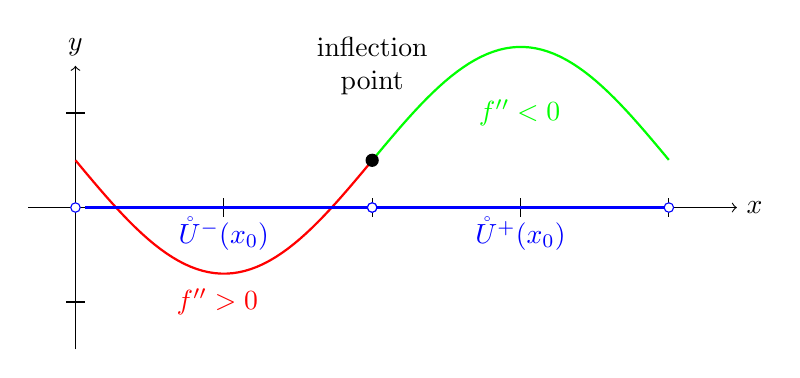
\begin{tikzpicture}[scale=1.2]
        % Draw coordinate axes
        \draw[->] (-0.5,0) -- (7,0) node[right] {$x$};
        \draw[->] (0,-1.5) -- (0,1.5) node[above] {$y$};
        
        % Draw the negative sine curve in two colors, shifted up by 0.5
        \draw[thick, red] plot[domain=0:3.14, samples=50] (\x, {-sin(\x r) * 1.2 + 0.5});
        \draw[thick, green] plot[domain=3.14:6.28, samples=50] (\x, {-sin(\x r) * 1.2 + 0.5});
        
        % Add second derivative labels
        \node[red] at (1.5,-1) {$f^{\prime\prime} > 0$};
        \node[green] at (4.7,1) {$f^{\prime\prime} < 0$};
        
        % Add inflection point label - updated y-coordinate to match the shift
        \fill (3.14,0.5) circle (0.07);
        \node[align=center] at (3.14,1.5) {inflection\\point};
        
        % Add key points on x-axis (ticks only, no labels)
        \foreach \x in {0, 1.57, 3.14, 4.71, 6.28} {
          \draw (\x,0.1) -- (\x,-0.1);
        }
        
        % Add blue intervals with hollow endpoints
        % First interval (0, pi)
        \draw[blue, thick] (0.1,0) -- (3.14,0);
        \draw[blue, fill=white] (0.0,0) circle (0.05);
        \draw[blue, fill=white] (3.14,0) circle (0.05);
        \node[blue, below] at (1.57,0) {$\mathring{U}^{-}(x_0)$};
        
        % Second interval (pi, 2pi)
        \draw[blue, thick] (3.14,0) -- (6.28,0);
        \draw[blue, fill=white] (3.14,0) circle (0.05);
        \draw[blue, fill=white] (6.28,0) circle (0.05);
        \node[blue, below] at (4.71,0) {$\mathring{U}^{+}(x_0)$};
        
        % Add key points on y-axis (ticks only, no labels)
        \foreach \y in {-1, 1} {
          \draw (0.1,\y) -- (-0.1,\y);
        }
      \end{tikzpicture}
      \caption{Curve with changing concavity and inflection point at $\pi$}
      \label{fig:neg-sine-concavity}
    \end{figure}
  \end{definition}

